\section{Reciprocal Consistency}
\label{sec:recipr-cons}

In the property graph data model, edges have direction and each edge runs from a \emph{source} vertex to a \emph{destination} vertex.
In the storage layer, however, edge directionality does not exist;  \textbf{both} the source and the destination vertices store information about each other.
This allows edge traversal to be bidirectional and speeds up query performance.

Consider, for example, the statement: ``Tolkien \textit{wrote} The Hobbit''.
It is expressed using vertex  \emph{a} for Tolkien and vertex \emph{b} for The Hobbit, and an edge \textit{wrote} running from \emph{a} (source) to \emph{b} (destination). Corresponding openCypher \cite{openCypher} code is given below and Fig \ref{rc-edge} shows the model level view.% of edge $ab$.
\begin{Verbatim}[commandchars=\\\{\},fontsize=\small,xleftmargin=.2in]
\textcolor{blue}{MATCH} (a:\textcolor{green}{Person}), (b:\textcolor{green}{Book})
\textcolor{blue}{WHERE} a.\textcolor{red}{name} = 'Tolkien' \textcolor{blue}{AND} b.\textcolor{red}{title} = 'The Hobbit'
\textcolor{blue}{CREATE} (a)-[w:\textcolor{green}{WROTE}]->(b)
\end{Verbatim}

Fig \ref{db-rep} depicts the internal representation of a graph arising from JanusGraph \cite{janusgraph} and TitanDB \cite{TitanDB}.
A vertex, such as \emph{a}, is represented by a record that contains one or more properties of that vertex, followed by a sequence of \emph{edge pointers} pointing to all those vertices to which this vertex is related either as a source or a destination.
The sequence of edge pointers is also called the \emph{adjacency list}.

It can be seen in Fig \ref{db-rep} that \emph{a}'s adjacency list has an edge pointer entry that stores `\emph{a} \emph{wrote} \emph{b}' while \emph{b}'s list has a corresponding entry storing the reciprocal (or inverse) information `\emph{b} \emph{written} by \emph{a}'.
When the adjacency list entries for a given edge refer to each other in a complementary manner like this, that edge is said to be \emph{reciprocally consistent}.

Consider a query: `list all titles by the author who wrote The Hobbit'.
This query needs to start from \emph{b} which represents the only entity specified explicitly in it.
Thanks to the reciprocal information in \emph{b}, it can reach \emph{a} from \emph{b}, even though edge \emph{ab} is  ``directed'' from \emph{a} to \emph{b}, and then compile the necessary list from \emph{a}.
Note that reciprocal consistency is assumed to be prevail when a query reads only the source or destination vertex of an edge.

\begin{figure}[htp]
  \centering
  \begin{subfigure}{\linewidth}
    \centering
    \begin{tikzpicture}[node distance=2.2cm]
  \node (v1) [big_vertex,xshift=0cm,yshift=0cm] {\small{\texttt{a:\textcolor{green}{Person}}}};
  \node (v2) [big_vertex,xshift=5cm,yshift=0cm] {\small{\texttt{b:\textcolor{green}{Book}}}};
  \node [below of=v1,yshift=1cm] {\small{\texttt{\textcolor{red}{name}:Tolkien}}};
  \node [below of=v2,yshift=1cm] {\small{\texttt{\textcolor{red}{title}:The Hobbit}}};
  \draw [thick,->,>=stealth] (0.9,0)  -- node [midway,above] {:\textcolor{green}{\small{\texttt{WROTE}}}} (4.1,0);
\end{tikzpicture}

    \caption{Logical view.}
    \label{rc-edge}
  \end{subfigure}
  %
  \begin{subfigure}{\linewidth}
    \vspace{2ex}
    \centering
    \begin{tikzpicture}[node distance=2cm,scale=0.6,every node/.style={transform shape}]

  \record(
  0,
  \small{\texttt{a:Person}},
  \small{\texttt{name:Tolkien}},
  $\boldsymbol{\rightarrow}$ \textbf{\small{\texttt{wrote b}}},
  \texttt{edge},
  \texttt{edge}
  );

  \record(
  -1,
  \small{\texttt{b:Book}},
  \texttt{property},
  \small{\texttt{title:The \hspace{-0.15cm} Hobbit}},
  $\boldsymbol{\leftarrow}$ \textbf{\small{\texttt{written by a}}},
  \texttt{edge}
  );

  \record(-2,
  \small{\texttt{vertex id}},
  \texttt{property},
  \texttt{property},
  \texttt{edge},
  \texttt{edge}
  );


  \spaceRecord(-3)

  \record(-4,
  \small{\texttt{vertex id}},
  \texttt{property},
  \texttt{edge},
  \texttt{edge},
  \texttt{edge}
  );

\end{tikzpicture}

    \caption{Storage view.}
    \label{db-rep}
  \end{subfigure}%
  \caption{Logical and storage views of a reciprocally consistent edge \emph{ab}.}
  \label{rc}
\end{figure}